\documentclass[12pt]{article}
%%% DOCUMENT FORMATTING %%%
\usepackage[margin=1in]{geometry}
\usepackage{enumitem}
\setlength{\parindent}{0pt}
\newcommand{\disp}{\displaystyle}

%%% HEADER %%%
\usepackage{fancyhdr}
\pagestyle{fancy}
\fancyhf{}
\lhead{MATH 1060}
\rhead{Vagnozzi}
\cfoot{\thepage}

%%% MATH NOTATION & SYMBOLS %%%
\usepackage{amssymb}
\usepackage{amsmath}
\newcommand{\R}{\mathbb{R}}
\newcommand{\N}{\mathbb{N}}
\newcommand{\Z}{\mathbb{Z}}
\newcommand{\lp}{\left(}
\newcommand{\rp}{\right)}
\newcommand{\ls}{\left[}
\newcommand{\rs}{\right]}
\newcommand{\lb}{\left\{}
\newcommand{\rb}{\right\}}
\newcommand{\arccot}{\text{arccot}}
\newcommand{\arccsc}{\text{arccsc}}
\newcommand{\arcsec}{\text{arcsec}} 

%%% TABLES %%%
\usepackage{colortbl}

%%% GRAPHS %%%
\usepackage{tikz}
\usepackage{pgfplots}
\pgfplotsset{compat=1.15}
\usepgfplotslibrary{fillbetween}
\usetikzlibrary{angles,quotes}

%%% ENVIRONMENTS %%%
\newcommand{\Example}{\paragraph{\Writinghand \hspace{0.1mm} Example.}}
\newcommand{\ExampleCont}{\paragraph{\Writinghand \hspace{0.1mm} Example (continued).}}
\newcommand{\boxenv}[2]{
	\fbox{
	\begin{minipage}{0.97\textwidth}
	\vspace{2mm}	
	\paragraph{#1} #2
	\vspace{2mm}
	\end{minipage}
	}}

%%% FUN THINGS %%%
\newcommand*\tc[1]{\tikz[baseline=(char.base)]{
            \node[shape=circle,draw,inner sep=2pt] (char) {#1};}}
\usepackage{marvosym}

%%% MISC %%%
\usepackage{hyperref}


\setcounter{page}{47}

\begin{document}
\section*{2.6: Continuity}

\boxenv{Learning Objectives.}{Upon successful completion of Section 2.6, you will be able to\dots
		
	\begin{itemize}[leftmargin=6mm]
		\item Answer conceptual questions involving continuity.
		\item Find points of discontinuity or intervals of continuity.
		\item Determine if functions are continuous at given values.
		\item Evaluate limits using continuity principles.
		\item Use the Intermediate Value Theorem to show equations have solutions on given \\ intervals.
		\item Sketch graphs of continuous functions given information about their points of \\ discontinuity.
		\item Solve applications involving continuity principles.
		\item Classify discontinuities.
	\end{itemize}
	\vspace{-4mm}
}

\vspace{5mm}

\subsection*{Introduction to Continuity}

Intuitively, a function is continuous if it is ``well-connected'' -- that is, it has no holes, breaks, gaps, or jumps. To begin our discussion of continuity, we introduce the idea of continuity at a point.

\vspace{3mm}

\boxenv{Definition.}{A function $f$ is \textbf{continuous at a point} $x=c$ if

\vspace{15mm}

If $f$ is not continuous at $x=c$, then we call $x=c$ a \textbf{point of discontinuity} and say that $f$ is \textbf{discontinuous} at $x=c$.}

\vspace{5mm}

This definition of continuity at a point implies three conditions that must simultaneously hold for a point $c$ in the domain of $f$.
\begin{itemize}
	\item[\tc{1}] $f(c)\in\R$
	\item[\tc{2}] $\disp\lim_{x\to c} f(x)$ exists
	\item[\tc{3}] $\disp\lim_{x\to c} f(x)=f(c)$
\end{itemize}

If any one of these conditions fails to hold, the function fails to be continuous at $x=c$. 

\newpage

\subsection*{Types of Discontinuities}

\paragraph{Removable Discontinuities.} Informally, we can think of removable continuities as minor holes in the graph that can be ``removed'' or ``fixed.''

\begin{center}
\begin{tikzpicture}[scale=1]
                \begin{axis}[
                	axis x line=middle,
                	xmax=2.2, xmin=-3.2,
                	axis y line=center,
                	ymax=2.5, ymin=-0.5,
                	xlabel=$x$,ylabel=$f$,
                	axis line style = {<->}
                    ]
                    \addplot[name path=f,smooth,domain=0:1.1,color=blue,samples=100,thick,->] {2*x^2};
                    \addplot[name path=f,smooth,domain=-2.15:0,color=blue,samples=100,thick,<-] {-(x+1)^2+1};
                    %\addplot[name path=f,smooth,domain=1:3,color=blue,samples=100,thick] {1};	
		    \addplot[mark=*,color=blue, fill=white] coordinates {(-1,1)};	
		    \addplot[mark=*,color=blue] coordinates {(-1,2)};	
		    %\addplot[mark=*,color=blue] coordinates {(1,1)};
		    %\addplot[mark=*,color=blue] coordinates {(3,1)};
		    %\addplot[mark=*,color=blue] coordinates {(2,2)};			
		    %\addplot[mark=*,color=blue,fill=white] coordinates {(1,2)};	
		    %\addplot[mark=*,color=blue,fill=white] coordinates {(1,3)};	
		    \addplot[mark=*,color=blue,fill=white] coordinates {(0,0)};
		    %\addplot[mark=*,color=blue,fill=white] coordinates {(2,1)};		
                \end{axis}
            \end{tikzpicture}
        \end{center}
        
If we do not have a graph available, we can still identify this type of discontinuity. A removable discontinuity will occur at $x=c$ when $\disp\lim_{x\to c}f(x)$ exists, but it is not equal to $f(c)$. 

\Example What type of discontinuity exists at $x=0$ for $f(x)=\disp\frac{x^2\cos x}{x^2 e^x+x^2}$?

\vspace{45mm}

\Example Redefine $f(x)=\disp\frac{x-1}{x^2-1}$ so it is continuous at $x=1$.

\newpage

\paragraph{Jump Discontinuities.} Jump discontinuities occur when a function approaches two different $y$-values as $x$ approaches a certain point. In other words, we can identify this type of discontinuity where the left- and right-hand limits are not equal to one another.

\begin{center}
            \begin{tikzpicture}
                \begin{axis}[
                	axis x line=middle,
                	xmax=4.2, xmin=-4.2,
                	axis y line=center,
                	ymax=2.2, ymin=-2.2,
                	xlabel=$x$,ylabel=$f$,
                	axis line style = {<->}
                    ]
                    \addplot[name path=f,smooth,domain=-3.9:1,color=blue,samples=100,thick,<-] {-1};
                    \addplot[name path=f,smooth,domain=1:3.9,color=blue,samples=100,thick,->] {1};
                    %\addplot[name path=f,smooth,domain=1:3,color=blue,samples=100,thick] {1};	
		   % \addplot[mark=*,color=blue] coordinates {(-1,1)};	
		    %\addplot[mark=*,color=blue] coordinates {(0,1)};	
		    %\addplot[mark=*,color=blue] coordinates {(1,1)};
		   % \addplot[mark=*,color=blue] coordinates {(3,1)};
		  %  \addplot[mark=*,color=blue] coordinates {(2,2)};			
		    \addplot[mark=*,color=blue,fill=white] coordinates {(1,-1)};	
		    \addplot[mark=*,color=blue,fill=white] coordinates {(1,1)};	
		   % \addplot[mark=*,color=blue,fill=white] coordinates {(0,0)};
		    %\addplot[mark=*,color=blue,fill=white] coordinates {(2,1)};		
                \end{axis}
            \end{tikzpicture}
        \end{center}


\paragraph{Infinite Discontinuities.} We have actually worked with infinite discontinuities before --- these are our vertical asymptotes.

\begin{center}
\begin{tikzpicture}
\begin{axis}[axis equal,axis x line=middle,
                	xmax=6.2, xmin=-6.2,
                	axis y line=center,
                	ymax=6.2, ymin=-6.2,
                	xlabel=$x$,ylabel=$f$,
                	axis line style = {<->}]
                    \addplot[name path=f,smooth,domain=3.25:7,color=blue,samples=100,thick,<->] {1/(x-3)+2};
                    \addplot[name path=f,smooth,domain=-7:2.65,color=blue,samples=100,thick,<->] {1/(x-3)-3};
    		    \draw [dashed,blue] (3,-6) -- (3,6);
    		    \draw [dashed,blue] (-8,2) -- (8,2);
    		    \draw [dashed,blue] (-8,-3) -- (8,-3);

\end{axis}
\end{tikzpicture}
        \end{center}
        
\vspace{5mm}

\subsection*{Continuity on an Interval}

\boxenv{Definition.}{A function $f$ is \textbf{right continuous} at $x=c$ if $\disp\lim_{x\to c^+}f(x)=f(c)$.

A function $f$ is \textbf{left continuous} at $x=c$ if $\disp\lim_{x\to c^-}f(x)= f(c)$.}

\vspace{3mm}

\boxenv{Definition.}{A function $f$ is \textbf{continuous on an interval} $\mathcal{I}$ if it is continuous (right, left, or both) for all $x\in\mathcal{I}$.}

\newpage 

\Example Identify the locations of discontinuities and classify them. Then determine the intervals for which the given function is continuous.

\begin{center}
            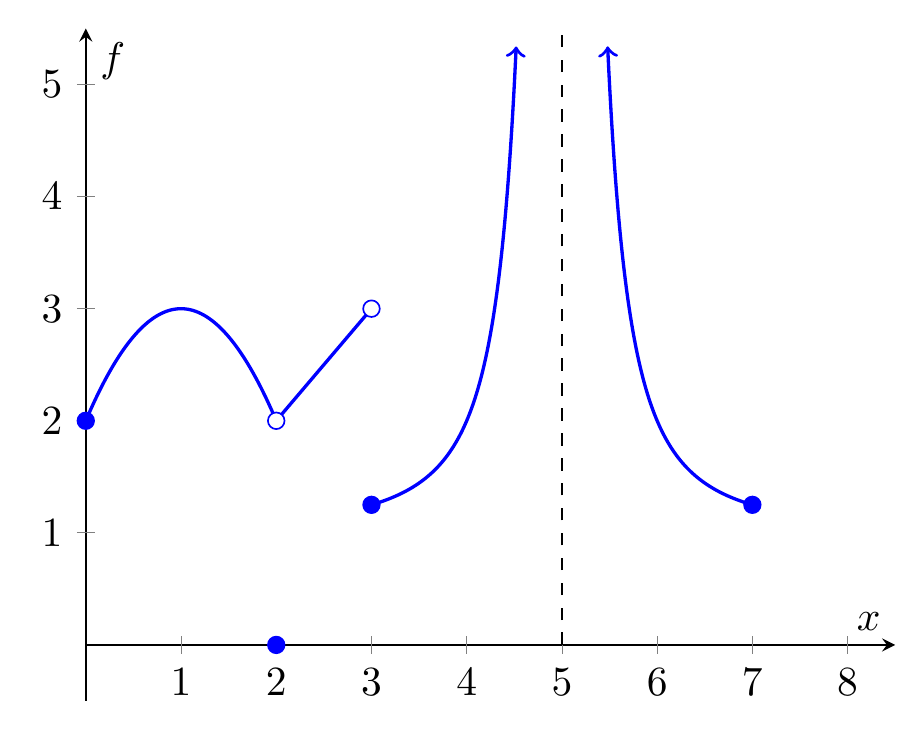
\begin{tikzpicture}[scale=1.5]
                \begin{axis}[
                	axis x line=middle,
                	xmax=8.5, xmin=0,
                	axis y line=center,
                	ymax=5.5, ymin=-0.5,
					xtick={\empty},
					extra x ticks={1,2,3,4,5,6,7,8},
					ytick={\empty},
					extra y ticks={1,2,3,4,5},
                	xlabel=$x$,ylabel=$f$
                    ]
                    \addplot[name path=f,smooth,domain=0:2,color=blue,samples=100,thick] {-(x-1)^2+3};
                    \addplot[name path=f,smooth,domain=2:3,color=blue,samples=100,thick] {x};
                    \addplot[name path=f,smooth,domain=3:4.52,color=blue,samples=100,thick,->] {(1/(x-5)^2)+1};	
                    \addplot[name path=f,smooth,domain=5.48:7,color=blue,samples=100,thick,<-] {(1/(x-5)^2)+1};	
		    \addplot[mark=*,color=blue] coordinates {(0,2)};
		    \addplot[mark=*,color=blue] coordinates {(7,1.25)};
		    \addplot[mark=*,color=blue] coordinates {(3,1.25)};
		    \addplot[mark=*,color=blue] coordinates {(2,0)};
																						
		    \addplot[mark=*,color=blue,fill=white] coordinates {(2,2)};	
		    \addplot[mark=*,color=blue,fill=white] coordinates {(3,3)};
		\draw [dashed] (5,0) -- (5,5.5);			
                \end{axis}
            \end{tikzpicture}
        \end{center}
        
\vspace{5mm}

\subsection*{Continuous Functions}

\boxenv{Definition.}{A function is called \textbf{continuous} if it is continuous (right, left, or both) for every $x$-value in its domain.}

\vspace{5mm}

You've worked with continuous functions before! The following functions are continuous.
\begin{itemize}
\item Polynomials
\item Rational Functions
\item Root functions
\item Trig and Inverse Trig Functions
\item Exponential and Logarithmic Functions
\end{itemize}        

Being familiar with types of functions that are continuous is valuable because you can use it as an argument to apply some of the tools and theorems from calculus.

\newpage

\Example Determine the intervals on which $f(x)=\disp\frac{x}{2x-5}$ is continuous. Classify any discontinuities.

\vspace{40mm}

\Example Determine the intervals on which $f(x)=\sqrt[4]{\ln x -2}$ is continuous.

\vspace{30mm}

\boxenv{Remark.}{Note the following two properties of continuous functions.
\begin{itemize}
	\item If $f$ is continuous and one-to-one, then $f^{-1}$ is continuous.
	\item If $f$ and $g$ are continuous, then $f\circ g$ and $g\circ f$ are continuous.
\end{itemize}

\vspace{-3mm}
}

\vspace{5mm}
This leads us to the following result for taking the limit of composite functions.

\vspace{3mm}

\boxenv{Theorem.}{If $g$ is continuous at $x=c$ and $f$ is continuous at $g(c)$, then
$$\lim_{x\to c}f\lp g(x)\rp=f\lp\lim_{x\to c}g(x)\rp.$$

\vspace{-5mm}}

\Example Evaluate the following limit.

\vspace{5mm}

\hspace{10mm} $\disp\lim_{x\to\infty} 2\cos\lp\frac{1}{2}\arctan x\rp$

\newpage

\subsection*{Intermediate Value Theorem (IVT)}

\boxenv{Intermediate Value Theorem.}{Suppose that $f$ is continuous on the closed interval $\ls a,b \rs$ with
$$f(a)\cdot f(b)<0\,\Longleftrightarrow\, f(a)\text{ and } f(b) \text{ differ in sign.}$$

\vspace{2mm}

Then there exists $x\in (a,b)$ such that $f(x)=0$.}

\begin{center}
            \begin{tikzpicture}
                \begin{axis}[
                	axis x line=middle,
                	xmax=pi, xmin=0,
                	axis y line=center,
                	ymax=1.2, ymin=-1.2,
                	xlabel=$x$,ylabel=$f$
                    ]
                    \addplot[name path=f,smooth,domain=0.5:2.75,color=blue,samples=100,thick] {cos(deg(x)};
		    \addplot[mark=*,color=blue] coordinates {(0.5,{cos(deg(0.5))})};
		    \addplot[mark=*,color=blue] coordinates {(2.75,{cos(deg(2.75))})};

                \end{axis}
            \end{tikzpicture}
        \end{center}
        
        \vspace{5mm}
        
Note that the converse of the Intermediate Value Theorem is not true. In other words, $f(a)\cdot f(b)>0$ does \underline{not} imply that there is \underline{not} a zero on $\ls a,b \rs$.

\begin{center}
            \begin{tikzpicture}
                \begin{axis}[
                	axis x line=middle,
                	xmax=2*pi, xmin=-0.25*pi,
                	axis y line=center,
                	ymax=1.2, ymin=-1.2,
                	xlabel=$x$,ylabel=$f$
                    ]
                    \addplot[name path=f,smooth,domain=0:2*pi,color=blue,samples=100,thick] {cos(deg(x))};
		    \addplot[mark=*,color=blue] coordinates {(0,1)};
		    \addplot[mark=*,color=blue] coordinates {(2*pi,1)};
		    \addplot[mark=x,color=red] coordinates {(0.5*pi,0)};
		    \addplot[mark=x,color=red] coordinates {(1.5*pi,0)};

                \end{axis}
            \end{tikzpicture}
        \end{center}
        
\newpage 

The graph below illustrates why continuity is critical to the Intermediate Value Theorem.

\begin{center}
            \begin{tikzpicture}
                \begin{axis}[
                	axis x line=middle,
                	xmax=2*pi, xmin=-pi,
                	axis y line=center,
                	ymax=1.2, ymin=-1.2,
                	xlabel=$x$,ylabel=$f$,
                	axis line style=<->
                    ]
                    \addplot[name path=f,smooth,domain=-1.4:1,color=blue,samples=200,thick,-] {cos(deg(x)};
                    \addplot[name path=f,smooth,domain=2:4.5,color=blue,samples=200,thick,-] {cos(deg(x)};
		    \addplot[mark=*,color=blue] coordinates {(1,{cos(deg(1))})};
		    \addplot[mark=*,color=blue] coordinates {(-1.4,{cos(deg(-1.4))})};

		    \addplot[mark=*,color=blue] coordinates {(2,{cos(deg(2))})};
		    \addplot[mark=*,color=blue] coordinates {(4.5,{cos(deg(4.5))})};

                \end{axis}
            \end{tikzpicture}
        \end{center}
        
        \vspace{5mm}
        
        
\Example Show that $f(x)=x^4+x-3$ has a zero between $x=1$ and $x=2$.
\end{document}